\chapter{Perancangan}
\label{chap:perancangan}

Bab ini membahas perancangan fitur Kolektor Pengumuman Informatika. Pembahasan dibagi menjadi tiga bagian, yaitu : perancangan kelas, perancangan basis data, dan perancangan antarmuka.
 
\section{Perancangan Kelas}
\begin{figure}[H]
	\centering  
	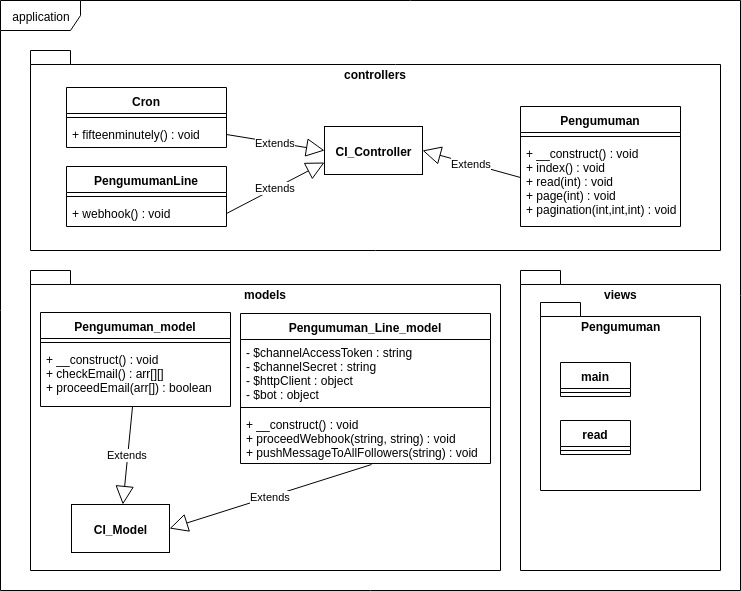
\includegraphics[width=\textwidth]{class-diagram.jpg}  
	\caption[Class diagram fitur Kolektor Pengumuman Informatika]{Class diagram fitur Kolektor Pengumuman Informatika} 
	\label{fig:class-diagram} 
\end{figure}
Gambar~\ref{fig:class-diagram} merupakan gambar diagram kelas yang dipakai untuk pembangunan fitur Kolektor Pengumuman Informatika. Penjelasan untuk diagram kelas tersebut akan diberikan di subbagian. Penjelasan dibagi menjadi tiga bagian : controller, model, dan view.

\subsection{Model}
Model yang digunakan ada dua, yaitu Pengumuman\_model dan Pengumuman\_Line\_model.
\subsubsection{Pengumuman\_model}
Pengumuman\_model berisi algoritma yang dibutuhkan oleh fitur Kolektor Pengumuman Informatika. Pengumuman\_model memiliki tiga method : \_\_construct, checkEmail, dan proceedEmail. Tabel \ref{table:pengumuman-model-construct}, \ref{table:pengumuman-model-checkemail}, dan \ref{table:pengumuman-model-proceedemail} menjelaskan secara rinci method-method tersebut.

\begin{center}
	\begin{table}[H]
	\caption{Rincian method \_\_construct}
	\label{table:pengumuman-model-construct}
\begin{tabular}{|c|p{11cm}|}
\hline
Nama Method 	& 	 	\_\_construct \\
\hline
Parameter Input & - \\
\hline
Parameter Output & - \\
\hline
Tabel yang berhubungan & -\\
\hline
Kelas yang berhubungan &  - \\
\hline
Deskripsi	& Method ini digunakan untuk konstruksi\\
\hline
Algoritma	& \begin{enumerate}
				\item Konstruksi dari parent.
				\item Load config auth dan modules.
				\end{enumerate} \\
\hline
\end{tabular}
\end{table}
\end{center}

\begin{center}
	\begin{table}[H]
	\caption{Rincian method checkEmail}
	\label{table:pengumuman-model-checkemail}
\begin{tabular}{|c|p{11cm}|}
\hline
Nama Method 	& 	 	checkEmail\\
\hline
Parameter Input & - \\
\hline
Parameter Output & Array dua dimensi. Dimensi pertama mewakili satu email, sedangkan dimensi kedua mewakili informasi dari email tersebut.\\
\hline
Tabel yang berhubungan & - \\
\hline
Kelas yang berhubungan & - \\
\hline
Deskripsi	& \\
\hline
Algoritma	& \begin{enumerate}
				\item Membuka koneksi imap ke email pengumuman.
				\item Mencari email yang belum dibaca.
				\item Apabila ada email yang belum dibaca, maka email tersebut dan informasinya dimasukkan ke dalam array.
				\item Menutup koneksi imap dan mengembalikan array.
				\end{enumerate} \\
\hline
\end{tabular}
\end{table}
\end{center}

\begin{center}
	\begin{table}[H]
	\caption{Rincian method proceedEmail}
	\label{table:pengumuman-model-proceedemail}
\begin{tabular}{|c|p{11cm}|}
\hline
Nama Method 	& 	 proceedEmail	\\
\hline
Parameter Input & Array asosiatif berisi informasi dari sebuah email. \\
\hline
Parameter Output & Mengembalikan true apabila email termasuk email pengumuman dan mengembalikan false apabila email tidak termasuk email pengumuman.  \\
\hline
Tabel yang berhubungan & Pengumuman \\
\hline
Kelas yang berhubungan &  Pengumuman\_Line\_model \\
\hline
Deskripsi	& Method ini berfungsi untuk memroses email pengumuman\\
\hline
Algoritma	& \begin{enumerate}
				\item load config pengumuman
				\item Memeriksa pengirim setiap email. Apabila pengirim terdaftar di config pengirimTerverifikasi, maka email tersebut akan masuk ke tahap berikutnya.
				\item Tahap berikutnya adalah memasukkan informasi email ke dalam baris record di tabel Pengumuuman dan mengirimkan pesan melalui Line. Pesan Line dikirimkan dengan bantuan method pushMessageToAllFollowers yang terdapat pada Pengumuman\_Line\_model.
				\item Mengembalikan true apabila sebelumnya email diidentifikasi sebagai  email pengumuman dan mengembalikan false apabila sebelumnya email diidentifikasi tidak termasuk email pengumuman.
				\end{enumerate} \\
\hline
\end{tabular}
\end{table}
\end{center}

\subsubsection{Pengumuman\_Line\_model}
Pengumuman\_Line\_model berisi algoritma yang dibutuhkan untuk berkomunikasi dengan Line API. Algoritma tersebut sengaja tidak disatukan ke dalam kelas Pengumuman\_model karena menggunakan banyak package tambahan dan memiliki atribut-atribut yang tidak dibutuhkan semua method yang berada di Pengumuman\_model. Atribut-atribut tersebut adalah : \textdollar channelAccessToken, \textdollar channelSecret, \textdollar httpClient, dan \textdollar bot. Pengumuman\_Line\_model memiliki tiga method : \_\_construct, proceedWebhook, dan pushMessageToAllFollowers. Tabel \ref{table:pengumuman-line-model-construct}, \ref{table:pengumuman-line-model-proceedwebhook}, dan \ref{table:pengumuman-line-model-pushmessagetoallfollowers} menjelaskan secara rinci method-method tersebut.

\begin{center}
	\begin{table}[H]
	\caption{Rincian method \_\_construct}
	\label{table:pengumuman-line-model-construct}
\begin{tabular}{|c|p{11cm}|}
\hline
Nama Method 	& 	 	\_\_construct \\
\hline
Parameter Input & - \\
\hline
Parameter Output & - \\
\hline
Tabel yang berhubungan & -\\
\hline
Kelas yang berhubungan &  - \\
\hline
Deskripsi	& Method ini digunakan untuk konstruksi\\
\hline
Algoritma	& \begin{enumerate}
				\item Konstruksi dari parent.
				\item Load config auth dan modules.
				\item Assign value untuk setiap atribut.
				\end{enumerate} \\
\hline
\end{tabular}
\end{table}
\end{center}

\begin{center}
	\begin{table}[H]
	\caption{Rincian method proceedWebhook}
	\label{table:pengumuman-line-model-proceedwebhook}
\begin{tabular}{|c|p{11cm}|}
\hline
Nama Method 	& 	 proceedWebhook	\\
\hline
Parameter Input & HTTP request body dan X Line Signature \\
\hline
Parameter Output & - \\
\hline
Tabel yang berhubungan & PengumumanLineFollowers\\
\hline
Kelas yang berhubungan & kelas-kelas di package LINE/LINEBot \\
\hline
Deskripsi	& Method ini untuk memproses event yang masuk ke dalam method webhook yang terdapat di PengumumanLine\\
\hline
Algoritma	& \begin{enumerate}
				\item Validasi signature dengan menggunakan method validateSignature yang membutuhkan parameter input HTTP request body dan X Line Signature.
				\item Jika signature valid, maka jenis event yang masuk akan dicek dan ditangani. Event yang wajib ditangani adalah FollowEvent dan UnfollowEvent. Apabila FollowEvent terjadi (ada user yang mengikuti bot atau membuka blokir bot), maka id user line tersebut akan dimasukkan ke tabel PengumumanLineFollowers. Apabila UnfollowEvent terjadi (ada user yang memblokir bot), maka id user line tersebut akan dihapus dari tabel PengumumanLineFollowers. Penyimpanan id user diperlukan untuk mengirim pesan ke pengikut bot.
				\end{enumerate} \\
\hline
\end{tabular}
\end{table}
\end{center}

\begin{center}
	\begin{table}[H]
	\caption{Rincian method pushMessageToAllFollowers}
	\label{table:pengumuman-line-model-pushmessagetoallfollowers}
\begin{tabular}{|c|p{11cm}|}
\hline
Nama Method 	& 	 pushMessageToAllFollowers	\\
\hline
Parameter Input & Pesan yang ingin dikirimkan ke pengikut bot \\
\hline
Parameter Output & - \\
\hline
Tabel yang berhubungan & PengumumanLineFollowers \\
\hline
Kelas yang berhubungan & kelas-kelas di package LINE/LINEBot \\
\hline
Deskripsi	& \\
\hline
Algoritma	& \begin{enumerate}
				\item Membuat query untuk mendapatkan semua id user line pengikut bot dan memasukkan hasilnya ke suatu array.
				\item Membuat text message builder dengan parameter input pesan yang ingin dikirimkan ke pengikut bot.
				\item Melakukan multicast dengan parameter input array id user line yang akan dikirimkan pesan dan text message builder.
				\end{enumerate} \\
\hline
\end{tabular}
\end{table}
\end{center}

\subsection{View}
View dibagi menjadi dua file php, yaitu main dan read. File main berfungsi untuk mengatur tampilan saat menampilkan daftar pengumuman. Sedangkan file read berfungsi untuk mengatur tampilan saat informasi dari satu email pengumuman ditampilkan.

\subsection{Controller}
Controller yang digunakan ada tiga, yaitu Cron, Pengumuman, dan PengumumanLine.
\subsubsection{Cron}
Controller Cron berfungsi untuk menjalankan perintah-perintah yang harus dijalankan pada jadwal tertentu. Method yang dimiliki hanya satu, yaitu : fifteenminutely(). Tabel \ref{table:cron-daily} menjelaskan secara rinci method fifteenminutely().

\begin{center}
	\begin{table}[H]
	\caption{Rincian method fifteenminutely}
	\label{table:cron-daily}
\begin{tabular}{|c|p{11cm}|}
\hline
Nama Method 	& 	fifteenminutely 	\\
\hline
Parameter Input & - \\
\hline
Parameter Output & - \\
\hline
Tabel yang berhubungan & - \\
\hline
Kelas yang berhubungan & Pengumuman\_model \\
\hline
Deskripsi	& Method yang perintah di dalamnya akan dijalankan setiap lima belas menit sekali. Untuk keperluan skripsi ini, method ini diisi dengan perintah untuk memeriksa email. Namun, apabila ada pengembangan lebih lanjut dan ada kebutuhan untuk menjalankan perintah setiap lima belas menit, maka isi method ini dapat ditambah.\\
\hline
Algoritma	& \begin{enumerate}
				\item Menjalankan method checkEmail() yang terdapat pada Pengumuman\_model.
				\item Memeriksa output dari Pengumuman\_model yang berupa array. Apabila tidak null, maka setiap elemen pada array tersebut akan dijadikan input dari method proceedEmail() yang terdapat pada Pengumuman\_model.
				\item Menjalankan method proceedEmail() yang terdapat pada Pengumuman\_model.
				\end{enumerate} \\
\hline
\end{tabular}
\end{table}
\end{center}

\subsubsection{Pengumuman}
Controller Pengumuman berfungsi untuk mengatur hubungan antara Pengumuman\_model dan view yang ada di package Pengumuman. Pengumuman\_model memiliki lima method, yaitu \_\_construct, index, read, page, dan pagination. Tabel \ref{table:pengumuman-construct}, \ref{table:pengumuman-index}, \ref{table:pengumuman-read}, \ref{table:pengumuman-page}, dan \ref{table:pengumuman-pagination} menjelaskan secara rinci method-method tersebut.

\begin{center}
	\begin{table}[H]
	\caption{Rincian method \_\_construct}
	\label{table:pengumuman-construct}
\begin{tabular}{|c|p{11cm}|}
\hline
Nama Method 	& 	 	\_\_construct \\
\hline
Parameter Input & - \\
\hline
Parameter Output & - \\
\hline
Tabel yang berhubungan & -\\
\hline
Kelas yang berhubungan &  - \\
\hline
Deskripsi	& Method ini digunakan untuk konstruksi\\
\hline
Algoritma	& \begin{enumerate}
				\item Konstruksi dari parent.
				\item Mengecek module yang diizinkan.
				\item Load library BlueTape
				\item Load model Pengumuman\_model
				\item load database
				\end{enumerate} \\
\hline
\end{tabular}
\end{table}
\end{center}

\begin{center}
	\begin{table}[H]
	\caption{Rincian method index}
	\label{table:pengumuman-index}
\begin{tabular}{|c|p{11cm}|}
\hline
Nama Method 	& 	 index	\\
\hline
Parameter Input & - \\
\hline
Parameter Output & - \\
\hline
Tabel yang berhubungan & Pengumuman \\
\hline
Kelas yang berhubungan & - \\
\hline
Deskripsi	& Mengatur halaman utama pengumuman\\
\hline
Algoritma	& \begin{enumerate}
				\item Mengambil info user
				\item Memasang link untuk setiap pengumuman yang ditampilkan pada daftar pengumuman.
				\item Menampilkan halaman pertama.
				\end{enumerate} \\
\hline
\end{tabular}
\end{table}
\end{center}

\begin{center}
	\begin{table}[H]
	\caption{Rincian method read}
	\label{table:pengumuman-read}
\begin{tabular}{|c|p{11cm}|}
\hline
Nama Method 	& 	 read	\\
\hline
Parameter Input & Id pengumuman \\
\hline
Parameter Output & - \\
\hline
Tabel yang berhubungan & Pengumuman \\
\hline
Kelas yang berhubungan & - \\
\hline
Deskripsi	& Mengatur halaman yang menampilkan detail pengumuman\\
\hline
Algoritma	& \begin{enumerate}
				\item Membuat query untuk mendapatkan seluruh informasi yang dimiliki oleh id pengumuman yang diinput dan memasukkannya ke suatu array.
				\item Load view untuk read dan oper array tersebut ke view.
				\end{enumerate} \\
\hline
\end{tabular}
\end{table}
\end{center}

\begin{center}
	\begin{table}[H]
	\caption{Rincian method page}
	\label{table:pengumuman-page}
\begin{tabular}{|c|p{11cm}|}
\hline
Nama Method 	& 	 page	\\
\hline
Parameter Input & nomor halaman yang ingin ditampilkan \\
\hline
Parameter Output & - \\
\hline
Tabel yang berhubungan & -\\
\hline
Kelas yang berhubungan & - \\
\hline
Deskripsi	& Menampilkan halaman pengumuman pada nomor halaman yang diinput.\\
\hline
Algoritma	& \begin{enumerate}
				\item Mengatur batas maksimal jumlah pengumuman yang ditampilkan pada satu halaman.
				\item Memanggil method pagination dengan input nomor halaman, batas tersebut, dan id pengumuman yang akan ditampilkan di baris pertama.
				\end{enumerate} \\
\hline
\end{tabular}
\end{table}
\end{center}

\begin{center}
	\begin{table}[H]
	\caption{Rincian method pagination}
	\label{table:pengumuman-pagination}
\begin{tabular}{|c|p{11cm}|}
\hline
Nama Method 	& 	 pagination	\\
\hline
Parameter Input &  Nomor halaman yang ingin ditampilkan, batas maksimal jumlah pengumuman yang ditampilkan pada satu halaman, dan id pengumuman yang akan ditampilkan di baris pertama.\\
\hline
Parameter Output & - \\
\hline
Tabel yang berhubungan & Pengumuman \\
\hline
Kelas yang berhubungan & - \\
\hline
Deskripsi	& Menampilkan halaman pengumuman pada nomor halaman yang diinput.\\
\hline
Algoritma	& \begin{enumerate}
				\item Membuat query untuk mengetahui jumlah pengumuman yang ada di tabel Pengumuman				
				\item Membuat query untuk mendapatkan informasi dari pengumuman yang akan tampil di halaman tersebut dan memasukkannya ke suatu array.
				\item Load view untuk main dan oper jumlah pengumuman yang ada di tabel Pengumuman, array tersebut, nomor halaman yang sedang ditampilkan, dan batas maksimal jumlah pengumuman yang ditampilkan pada satu halaman ke view.
				\end{enumerate} \\
\hline
\end{tabular}
\end{table}
\end{center}

\subsubsection{PengumumanLine}
Controller PengumumanLine berfungsi untuk menerima webhook dari LineAPI. PengumumanLine memiliki satu method yaitu webhook. Method ini sengaja dipisah dari controller Pengumuman karena proteksi csrf perlu dibuka untuk menerima webhook. Tabel \ref{table:pengumumanline-webhook} menjelaskan method tersebut secara rinci.

\begin{center}
	\begin{table}[H]
	\caption{Rincian method webhook}
	\label{table:pengumumanline-webhook}
\begin{tabular}{|c|p{11cm}|}
\hline
Nama Method 	& 	 webhook	\\
\hline
Parameter Input & Request berisi event dari Line API melalui POST \\
\hline
Parameter Output & - \\
\hline
Tabel yang berhubungan & -\\
\hline
Kelas yang berhubungan & Pengumuman\_Line\_model \\
\hline
Deskripsi	& Method ini berfungsi untuk menerima request berisi event dari Line API melalui POST\\
\hline
Algoritma	& \begin{enumerate}
				\item Memeriksa apakah request yang masuk melalui POST. Jika tidak, maka akan mengembalikan http response code 405.
				\item Mengambil request yang masuk dan menyimpannya ke suatu variabel.
				\item Memeriksa apakah ada HTTP\_X\_LINE\_SIGNATURE pada POST yang masuk. Jika tidak ada, maka akan mengembalikan http response code 400.
				\item Jika ada, maka jalankan method proceedWebhook dengan parameter input variabel yang berisi request body dan X Line Signature.
				\end{enumerate} \\
\hline
\end{tabular}
\end{table}
\end{center}

\section{Perancangan Basis Data}
Tabel-tabel yang sudah ada di BlueTape tidak diubah, namun ada dua tabel yang ditambahkan. Kedua tabel tersebut adalah tabel Pengumuman dan tabel Line\_followers. Tabel pengumuman berguna untuk menyimpan informasi dari email pengumuman. Sedangkan tabel Line\_followers berguna untuk menyimpan user id dari follower akun bot BlueTape.

\subsubsection{Tabel Pengumuman}
\begin{center}
	\begin{table}[H]
	\caption{Perancangan Tabel Pengumuman}
	\begin{tabular}{|c|c|c|c|c|c|}
 			\hline
			\textbf{Atribut} & \textbf{Tipe Data} & \textbf{Constraint} & \textbf{PK*}  & \textbf{FK*} \\
			\hline
		 	 id & int & - & Ya & Tidak\\
			\hline
			 namaPengirim & VARCHAR & 256 & Tidak & Tidak\\
            \hline
			 emailPengirim & VARCHAR & 256 & Tidak & Tidak\\
            \hline
			 waktuTerkirim & timestamp & - & Tidak & Tidak\\
            \hline
			 subjek & VARCHAR & 256 & Tidak & Tidak\\
            \hline
			 isi & TEXT & 256 & Tidak & Tidak\\
            \hline
			 ketersediaanLampiran & VARCHAR & 1 & Tidak & Tidak\\
			\hline
	\end{tabular}
	\end{table}
\end{center}
\textit{*PK = Primary Key} \\
\textit{*FK = Foreign Key} \\

Keterangan atribut :
\begin{itemize}
\item \textbf{id} : Id pengumuman. Auto increment.
\item \textbf{namaPengirim} : Nama pengirim email pengumuman.
\item \textbf{emailPengirim} : Alamat email pengirim email pengumuman.
\item \textbf{waktuTerkirim} : Waktu terkirim email pengumuman.
\item \textbf{subjek} : Subjek email pengumuman.
\item \textbf{isi} : Isi email pengumuman. Boleh kosong.
\item \textbf{ketersediaanLampiran} : Jika email pengumuman memiliki lampiran maka atribut ini memiliki value 'Y'. Jika tidak, maka valuenya 'N'.
\end{itemize}

\subsubsection{Tabel PengumumanLineFollowers}
\begin{center}
	\begin{table}[H]
	\caption{Perancangan Tabel PengumumanLineFollowers}
	\begin{tabular}{|c|c|c|c|c|c|}
 			\hline
			\textbf{Atribut} & \textbf{Tipe Data} & \textbf{Constraint} & \textbf{PK*}  & \textbf{FK*} \\
			\hline
			 userId & VARCHAR & 256 & Ya & Tidak\\
            \hline
	\end{tabular}
	\end{table}
\end{center}
\textit{*PK = Primary Key} \\
\textit{*FK = Foreign Key} \\

Keterangan atribut :
\begin{itemize}
\item \textbf{userId} : User id dari akun LINE yang follow akun bot BlueTape.
\end{itemize}

\section{Perancangan Antarmuka}
	Bagian ini membahas perancangan antarmuka untuk fitur Kolektor Pengumuman Informatika pada BlueTape dan bot BlueTape.
\subsection{Perancangan Antarmuka pada BlueTape}
Antarmuka yang digunakan fitur Kolektor Pengumuman Informatika ada dua, yaitu main dan read. Penjelasan untuk desain kedua antarmuka tersebut terdapat di subbagian.

\subsubsection{main}

\begin{figure}[H]
	\centering  
	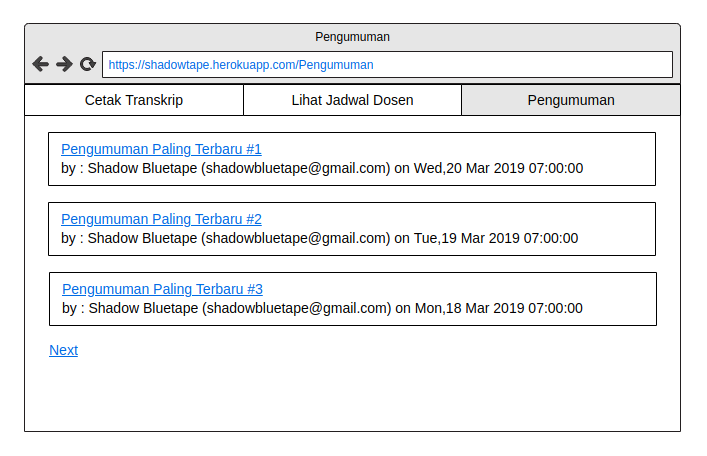
\includegraphics[width=\textwidth]{Mockup-main.png}  
	\caption[Mockup antarmuka main]{Mockup antarmuka main} 
	\label{fig:mockup-main} 
\end{figure}

Antarmuka main menampilkan daftar pengumuman. Jumlah pengumuman yang ditampilkan di satu halaman dibatasi pada angka tertentu. Di halaman main terdapat navigasi next dan prev untuk menampilkan daftar selanjutnya dan sesudahnya. Gambar~ \ref{fig:mockup-main} menampilkan mockup antarmuka main.

\subsubsection{read}

\begin{figure}[H]
	\centering  
	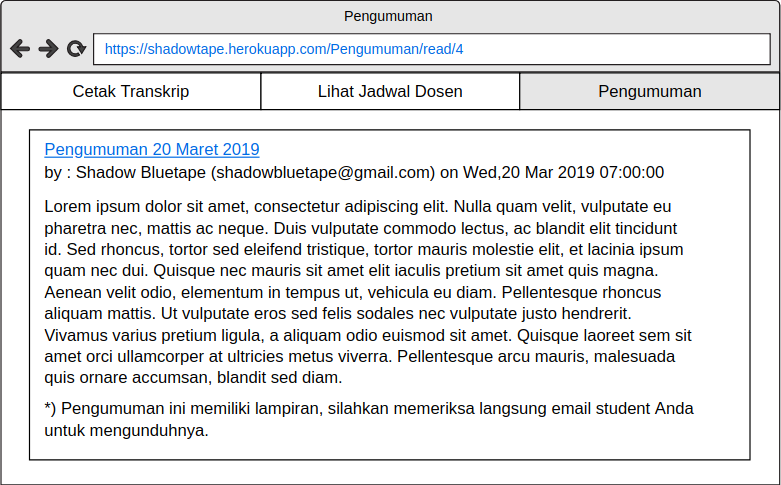
\includegraphics[width=\textwidth]{Mockup-read.png}  
	\caption[Mockup antarmuka read]{Mockup antarmuka read} 
	\label{fig:mockup-main} 
\end{figure}

Antarmuka main menampilkan informasi detil dari pengumuman. Apabila pengumuman memiliki lampiran, maka tulisan "*) Pengumuman ini memiliki lampiran, silahkan memeriksa langsung email student Anda untuk mengunduhnya." akan muncul. Jika tidak ada, maka tulisan tersebut tidak akan muncul. Gambar~ \ref{fig:mockup-main} menampilkan mockup antarmuka read.

\subsection{Perancangan Antarmuka pada Bot BlueTape}

\begin{figure}[H]
	\centering  
	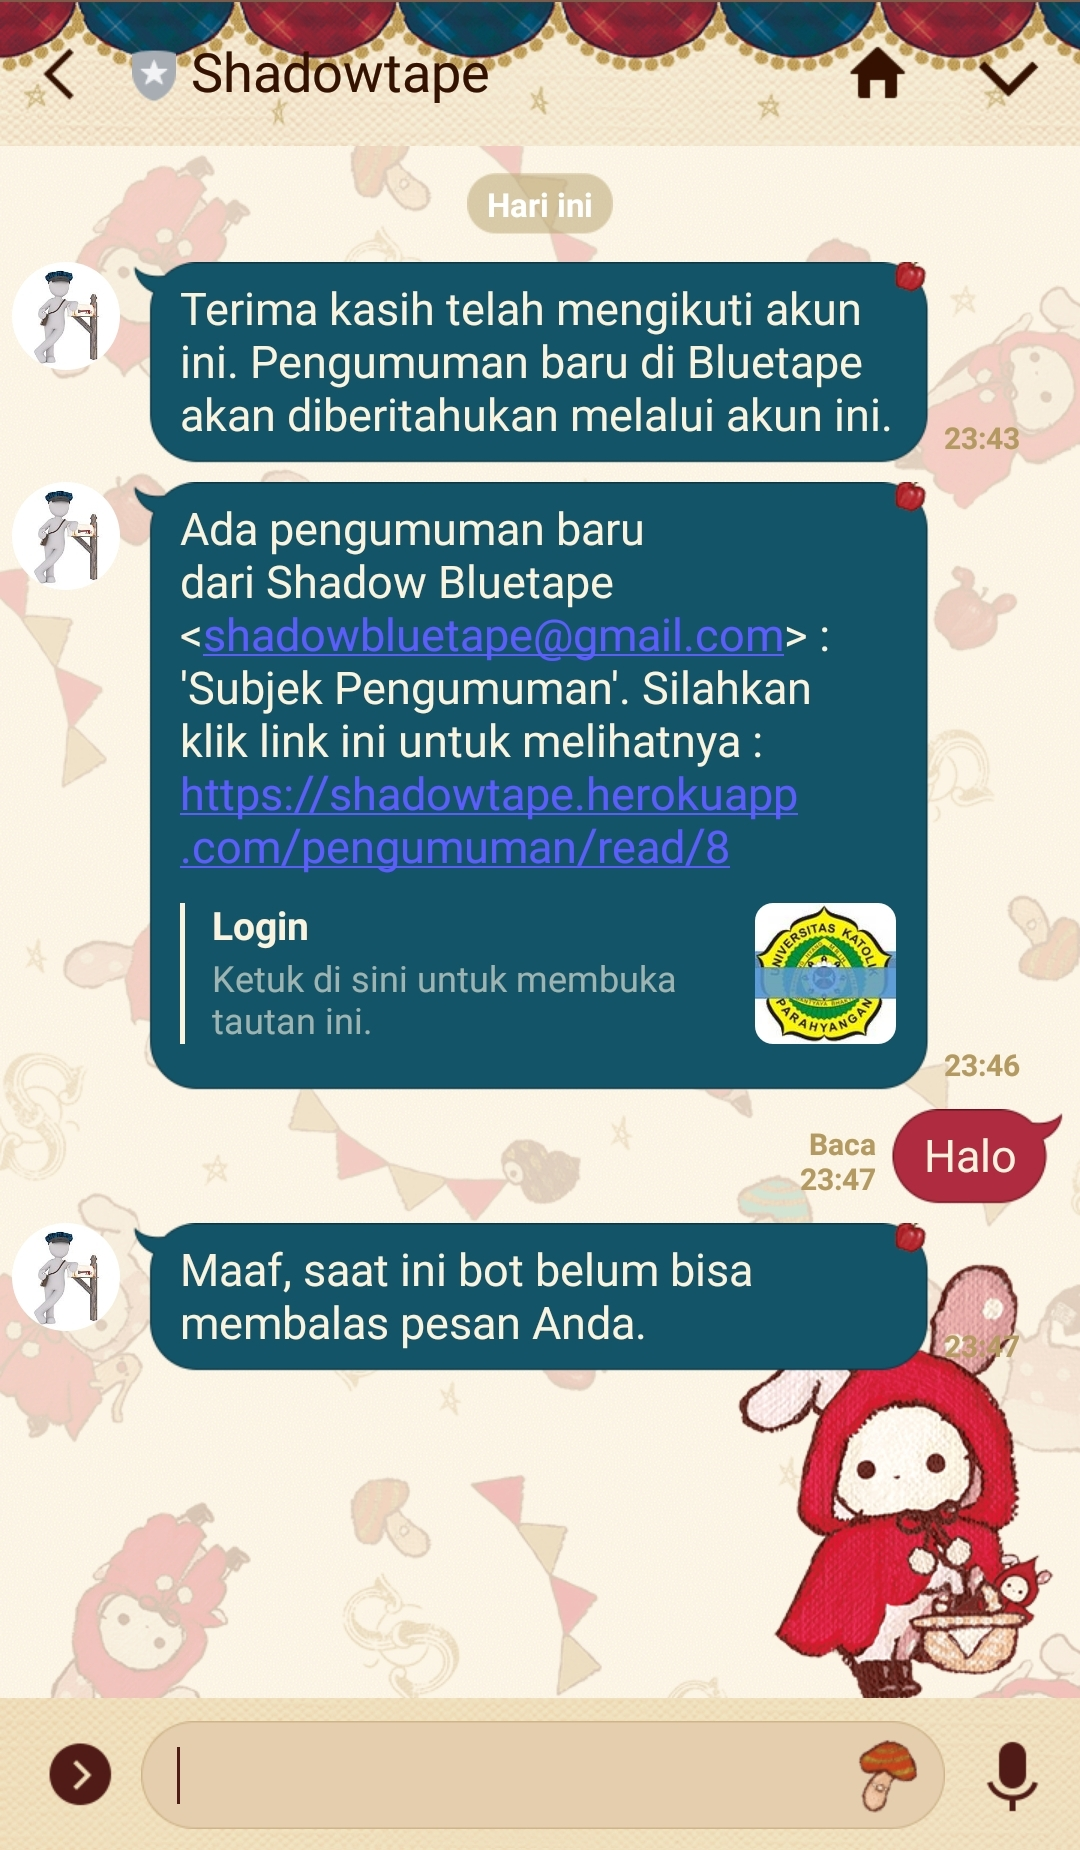
\includegraphics[width=\textwidth]{Mockup-bot.jpg}  
	\caption[Mockup antarmuka read]{Mockup antarmuka bot BlueTape} 
	\label{fig:mockup-bot} 
\end{figure}

Gambar~ \ref{fig:mockup-main} menampilkan mockup antarmuka bot BlueTape. Chat pertama merupakan pesan yang akan ditampilkan saat user baru mengikuti bot atau membuka blokir bot. Chat kedua merupakan contoh pesan yang akan ditampilkan jika ada pengumuman baru yang masuk ke BlueTape. Chat terakhir merupakan pesan balasan jika user mengirimkan pesan ke bot dalam bentuk apapun (teks, sticker, gambar, video, dan suara).